
%% bare_conf.tex
%% V1.3
%% 2007/01/11
%% by Michael Shell
%% See:
%% http://www.michaelshell.org/
%% for current contact information.
%%
%% This is a skeleton file demonstrating the use of IEEEtran.cls
%% (requires IEEEtran.cls version 1.7 or later) with an IEEE conference paper.
%%
%% Support sites:
%% http://www.michaelshell.org/tex/ieeetran/
%% http://www.ctan.org/tex-archive/macros/latex/contrib/IEEEtran/
%% and
%% http://www.ieee.org/

%%*************************************************************************
%% Legal Notice:
%% This code is offered as-is without any warranty either expressed or
%% implied; without even the implied warranty of MERCHANTABILITY or
%% FITNESS FOR A PARTICULAR PURPOSE! 
%% User assumes all risk.
%% In no event shall IEEE or any contributor to this code be liable for
%% any damages or losses, including, but not limited to, incidental,
%% consequential, or any other damages, resulting from the use or misuse
%% of any information contained here.
%%
%% All comments are the opinions of their respective authors and are not
%% necessarily endorsed by the IEEE.
%%
%% This work is distributed under the LaTeX Project Public License (LPPL)
%% ( http://www.latex-project.org/ ) version 1.3, and may be freely used,
%% distributed and modified. A copy of the LPPL, version 1.3, is included
%% in the base LaTeX documentation of all distributions of LaTeX released
%% 2003/12/01 or later.
%% Retain all contribution notices and credits.
%% ** Modified files should be clearly indicated as such, including  **
%% ** renaming them and changing author support contact information. **
%%
%% File list of work: IEEEtran.cls, IEEEtran_HOWTO.pdf, bare_adv.tex,
%%                    bare_conf.tex, bare_jrnl.tex, bare_jrnl_compsoc.tex
%%*************************************************************************

% *** Authors should verify (and, if needed, correct) their LaTeX system  ***
% *** with the testflow diagnostic prior to trusting their LaTeX platform ***
% *** with production work. IEEE's font choices can trigger bugs that do  ***
% *** not appear when using other class files.                            ***
% The testflow support page is at:
% http://www.michaelshell.org/tex/testflow/



% Note that the a4paper option is mainly intended so that authors in
% countries using A4 can easily print to A4 and see how their papers will
% look in print - the typesetting of the document will not typically be
% affected with changes in paper size (but the bottom and side margins will).
% Use the testflow package mentioned above to verify correct handling of
% both paper sizes by the user's LaTeX system.
%
% Also note that the "draftcls" or "draftclsnofoot", not "draft", option
% should be used if it is desired that the figures are to be displayed in
% draft mode.
%
\documentclass[10pt, conference, compsocconf]{IEEEtran}
% Add the compsocconf option for Computer Society conferences.
%
% If IEEEtran.cls has not been installed into the LaTeX system files,
% manually specify the path to it like:
% \documentclass[conference]{../sty/IEEEtran}





% Some very useful LaTeX packages include:
% (uncomment the ones you want to load)


% *** MISC UTILITY PACKAGES ***
%
%\usepackage{ifpdf}
% Heiko Oberdiek's ifpdf.sty is very useful if you need conditional
% compilation based on whether the output is pdf or dvi.
% usage:
% \ifpdf
%   % pdf code
% \else
%   % dvi code
% \fi
% The latest version of ifpdf.sty can be obtained from:
% http://www.ctan.org/tex-archive/macros/latex/contrib/oberdiek/
% Also, note that IEEEtran.cls V1.7 and later provides a builtin
% \ifCLASSINFOpdf conditional that works the same way.
% When switching from latex to pdflatex and vice-versa, the compiler may
% have to be run twice to clear warning/error messages.






% *** CITATION PACKAGES ***
%
%\usepackage{cite}
% cite.sty was written by Donald Arseneau
% V1.6 and later of IEEEtran pre-defines the format of the cite.sty package
% \cite{} output to follow that of IEEE. Loading the cite package will
% result in citation numbers being automatically sorted and properly
% "compressed/ranged". e.g., [1], [9], [2], [7], [5], [6] without using
% cite.sty will become [1], [2], [5]--[7], [9] using cite.sty. cite.sty's
% \cite will automatically add leading space, if needed. Use cite.sty's
% noadjust option (cite.sty V3.8 and later) if you want to turn this off.
% cite.sty is already installed on most LaTeX systems. Be sure and use
% version 4.0 (2003-05-27) and later if using hyperref.sty. cite.sty does
% not currently provide for hyperlinked citations.
% The latest version can be obtained at:
% http://www.ctan.org/tex-archive/macros/latex/contrib/cite/
% The documentation is contained in the cite.sty file itself.






% *** GRAPHICS RELATED PACKAGES ***
%
\ifCLASSINFOpdf
  \usepackage[pdftex]{graphicx}
  % declare the path(s) where your graphic files are
  %\graphicspath{{../pdf/}{../jpeg/}}
  % and their extensions so you won't have to specify these with
  % every instance of \includegraphics
  \DeclareGraphicsExtensions{.pdf,.jpeg,.png}
\else
  % or other class option (dvipsone, dvipdf, if not using dvips). graphicx
  % will default to the driver specified in the system graphics.cfg if no
  % driver is specified.
  % \usepackage[dvips]{graphicx}
  % declare the path(s) where your graphic files are
  % \graphicspath{{../eps/}}
  % and their extensions so you won't have to specify these with
  % every instance of \includegraphics
  % \DeclareGraphicsExtensions{.eps}
\fi
% graphicx was written by David Carlisle and Sebastian Rahtz. It is
% required if you want graphics, photos, etc. graphicx.sty is already
% installed on most LaTeX systems. The latest version and documentation can
% be obtained at: 
% http://www.ctan.org/tex-archive/macros/latex/required/graphics/
% Another good source of documentation is "Using Imported Graphics in
% LaTeX2e" by Keith Reckdahl which can be found as epslatex.ps or
% epslatex.pdf at: http://www.ctan.org/tex-archive/info/
%
% latex, and pdflatex in dvi mode, support graphics in encapsulated
% postscript (.eps) format. pdflatex in pdf mode supports graphics
% in .pdf, .jpeg, .png and .mps (metapost) formats. Users should ensure
% that all non-photo figures use a vector format (.eps, .pdf, .mps) and
% not a bitmapped formats (.jpeg, .png). IEEE frowns on bitmapped formats
% which can result in "jaggedy"/blurry rendering of lines and letters as
% well as large increases in file sizes.
%
% You can find documentation about the pdfTeX application at:
% http://www.tug.org/applications/pdftex





% *** MATH PACKAGES ***
%
%\usepackage[cmex10]{amsmath}
% A popular package from the American Mathematical Society that provides
% many useful and powerful commands for dealing with mathematics. If using
% it, be sure to load this package with the cmex10 option to ensure that
% only type 1 fonts will utilized at all point sizes. Without this option,
% it is possible that some math symbols, particularly those within
% footnotes, will be rendered in bitmap form which will result in a
% document that can not be IEEE Xplore compliant!
%
% Also, note that the amsmath package sets \interdisplaylinepenalty to 10000
% thus preventing page breaks from occurring within multiline equations. Use:
%\interdisplaylinepenalty=2500
% after loading amsmath to restore such page breaks as IEEEtran.cls normally
% does. amsmath.sty is already installed on most LaTeX systems. The latest
% version and documentation can be obtained at:
% http://www.ctan.org/tex-archive/macros/latex/required/amslatex/math/





% *** SPECIALIZED LIST PACKAGES ***
%
%\usepackage{algorithmic}
% algorithmic.sty was written by Peter Williams and Rogerio Brito.
% This package provides an algorithmic environment fo describing algorithms.
% You can use the algorithmic environment in-text or within a figure
% environment to provide for a floating algorithm. Do NOT use the algorithm
% floating environment provided by algorithm.sty (by the same authors) or
% algorithm2e.sty (by Christophe Fiorio) as IEEE does not use dedicated
% algorithm float types and packages that provide these will not provide
% correct IEEE style captions. The latest version and documentation of
% algorithmic.sty can be obtained at:
% http://www.ctan.org/tex-archive/macros/latex/contrib/algorithms/
% There is also a support site at:
% http://algorithms.berlios.de/index.html
% Also of interest may be the (relatively newer and more customizable)
% algorithmicx.sty package by Szasz Janos:
% http://www.ctan.org/tex-archive/macros/latex/contrib/algorithmicx/




% *** ALIGNMENT PACKAGES ***
%
%\usepackage{array}
% Frank Mittelbach's and David Carlisle's array.sty patches and improves
% the standard LaTeX2e array and tabular environments to provide better
% appearance and additional user controls. As the default LaTeX2e table
% generation code is lacking to the point of almost being broken with
% respect to the quality of the end results, all users are strongly
% advised to use an enhanced (at the very least that provided by array.sty)
% set of table tools. array.sty is already installed on most systems. The
% latest version and documentation can be obtained at:
% http://www.ctan.org/tex-archive/macros/latex/required/tools/


%\usepackage{mdwmath}
%\usepackage{mdwtab}
% Also highly recommended is Mark Wooding's extremely powerful MDW tools,
% especially mdwmath.sty and mdwtab.sty which are used to format equations
% and tables, respectively. The MDWtools set is already installed on most
% LaTeX systems. The lastest version and documentation is available at:
% http://www.ctan.org/tex-archive/macros/latex/contrib/mdwtools/


% IEEEtran contains the IEEEeqnarray family of commands that can be used to
% generate multiline equations as well as matrices, tables, etc., of high
% quality.


%\usepackage{eqparbox}
% Also of notable interest is Scott Pakin's eqparbox package for creating
% (automatically sized) equal width boxes - aka "natural width parboxes".
% Available at:
% http://www.ctan.org/tex-archive/macros/latex/contrib/eqparbox/



\ifCLASSOPTIONcompsoc
	\usepackage[caption=false,font=normalsize,labelfont=sf,textfont=sf]{subfig}
\else
	\usepackage[caption=false,font=footnotesize]{subfig}
\fi
% *** SUBFIGURE PACKAGES ***
%\usepackage[tight,footnotesize]{subfigure}
% subfigure.sty was written by Steven Douglas Cochran. This package makes it
% easy to put subfigures in your figures. e.g., "Figure 1a and 1b". For IEEE
% work, it is a good idea to load it with the tight package option to reduce
% the amount of white space around the subfigures. subfigure.sty is already
% installed on most LaTeX systems. The latest version and documentation can
% be obtained at:
% http://www.ctan.org/tex-archive/obsolete/macros/latex/contrib/subfigure/
% subfigure.sty has been superceeded by subfig.sty.



%\usepackage[caption=false]{caption}
%\usepackage[font=footnotesize]{subfig}
% subfig.sty, also written by Steven Douglas Cochran, is the modern
% replacement for subfigure.sty. However, subfig.sty requires and
% automatically loads Axel Sommerfeldt's caption.sty which will override
% IEEEtran.cls handling of captions and this will result in nonIEEE style
% figure/table captions. To prevent this problem, be sure and preload
% caption.sty with its "caption=false" package option. This is will preserve
% IEEEtran.cls handing of captions. Version 1.3 (2005/06/28) and later 
% (recommended due to many improvements over 1.2) of subfig.sty supports
% the caption=false option directly:
%\usepackage[caption=false,font=footnotesize]{subfig}
%
% The latest version and documentation can be obtained at:
% http://www.ctan.org/tex-archive/macros/latex/contrib/subfig/
% The latest version and documentation of caption.sty can be obtained at:
% http://www.ctan.org/tex-archive/macros/latex/contrib/caption/




% *** FLOAT PACKAGES ***
%
%\usepackage{fixltx2e}
% fixltx2e, the successor to the earlier fix2col.sty, was written by
% Frank Mittelbach and David Carlisle. This package corrects a few problems
% in the LaTeX2e kernel, the most notable of which is that in current
% LaTeX2e releases, the ordering of single and double column floats is not
% guaranteed to be preserved. Thus, an unpatched LaTeX2e can allow a
% single column figure to be placed prior to an earlier double column
% figure. The latest version and documentation can be found at:
% http://www.ctan.org/tex-archive/macros/latex/base/



%\usepackage{stfloats}
% stfloats.sty was written by Sigitas Tolusis. This package gives LaTeX2e
% the ability to do double column floats at the bottom of the page as well
% as the top. (e.g., "\begin{figure*}[!b]" is not normally possible in
% LaTeX2e). It also provides a command:
%\fnbelowfloat
% to enable the placement of footnotes below bottom floats (the standard
% LaTeX2e kernel puts them above bottom floats). This is an invasive package
% which rewrites many portions of the LaTeX2e float routines. It may not work
% with other packages that modify the LaTeX2e float routines. The latest
% version and documentation can be obtained at:
% http://www.ctan.org/tex-archive/macros/latex/contrib/sttools/
% Documentation is contained in the stfloats.sty comments as well as in the
% presfull.pdf file. Do not use the stfloats baselinefloat ability as IEEE
% does not allow \baselineskip to stretch. Authors submitting work to the
% IEEE should note that IEEE rarely uses double column equations and
% that authors should try to avoid such use. Do not be tempted to use the
% cuted.sty or midfloat.sty packages (also by Sigitas Tolusis) as IEEE does
% not format its papers in such ways.





% *** PDF, URL AND HYPERLINK PACKAGES ***
%
%\usepackage{url}
% url.sty was written by Donald Arseneau. It provides better support for
% handling and breaking URLs. url.sty is already installed on most LaTeX
% systems. The latest version can be obtained at:
% http://www.ctan.org/tex-archive/macros/latex/contrib/misc/
% Read the url.sty source comments for usage information. Basically,
% \url{my_url_here}.





% *** Do not adjust lengths that control margins, column widths, etc. ***
% *** Do not use packages that alter fonts (such as pslatex).         ***
% There should be no need to do such things with IEEEtran.cls V1.6 and later.
% (Unless specifically asked to do so by the journal or conference you plan
% to submit to, of course. )
\usepackage{listings}
\usepackage{color}
\usepackage{courier}

% correct bad hyphenation here
\hyphenation{op-tical net-works semi-conduc-tor}


\begin{document}
%
% paper title
% can use linebreaks \\ within to get better formatting as desired
\title{Achieving High-Throughput Distributed, Graph-based Multi-stage Stream Processing}


% author names and affiliations
% use a multiple column layout for up to two different
% affiliations

\author{\IEEEauthorblockN{Amila Suriarachchi}
\IEEEauthorblockA{Department of Computer Science\\
Colorado State University\\
Fort Collins, Colorado\\
amilas@cs.colostate.edu}
\and
\IEEEauthorblockN{Shrideep Pallickara}
\IEEEauthorblockA{Department of Computer Science\\
Colorado State University\\
Fort Collins, Colorado\\
shrideep@cs.colostate.edu}
}

% conference papers do not typically use \thanks and this command
% is locked out in conference mode. If really needed, such as for
% the acknowledgment of grants, issue a \IEEEoverridecommandlockouts
% after \documentclass

% for over three affiliations, or if they all won't fit within the width
% of the page, use this alternative format:
% 
%\author{\IEEEauthorblockN{Michael Shell\IEEEauthorrefmark{1},
%Homer Simpson\IEEEauthorrefmark{2},
%James Kirk\IEEEauthorrefmark{3}, 
%Montgomery Scott\IEEEauthorrefmark{3} and
%Eldon Tyrell\IEEEauthorrefmark{4}}
%\IEEEauthorblockA{\IEEEauthorrefmark{1}School of Electrical and Computer Engineering\\
%Georgia Institute of Technology,
%Atlanta, Georgia 30332--0250\\ Email: see http://www.michaelshell.org/contact.html}
%\IEEEauthorblockA{\IEEEauthorrefmark{2}Twentieth Century Fox, Springfield, USA\\
%Email: homer@thesimpsons.com}
%\IEEEauthorblockA{\IEEEauthorrefmark{3}Starfleet Academy, San Francisco, California 96678-2391\\
%Telephone: (800) 555--1212, Fax: (888) 555--1212}
%\IEEEauthorblockA{\IEEEauthorrefmark{4}Tyrell Inc., 123 Replicant Street, Los Angeles, California 90210--4321}}




% use for special paper notices
%\IEEEspecialpapernotice{(Invited Paper)}




% make the title area
\maketitle


\begin{abstract}
MapReduce \cite{dean2008mapreduce} is widely used to process offline data with the popularity of Apache Hadoop \cite{hadoop}. However the latencies introduced by the MapReduce frameworks are not suitable for unbounded continuous data stream processing. Firstly communication through the file system introduces higher delays compared to direct TCP stream communication and secondly synchronization delay between \textit{map} and \textit{reduce} jobs adds unnecessary delays for high volume stream data processing. In order to handle these issues distributed stream processing systems have been developed.


Although high performance is one of the main goals of those systems, there is less attention has been paid for inter node communication performance. Most of these frameworks do not explore the parallelism by making more parallel connections among nodes. Further some systems do not use efficient message serialization techniques which save the network bandwidth. In this paper we introduce a high performance inter node communication design which explore the parallelism and serialize and parse messages efficiently to optimize the throughput.


First we compare performance of our solution with Twitter storm \cite{twitterStorm} and  Yahoo S4 \cite{neumeyer2010s4} using an implementation of Pan Tompkins algorithm \cite{kohler2002principles} which is used to detect QRS complexities of an ECG signal using a 2 node graph. Our results show our solution performs 4x times better than other systems. Then we use 4 level node graph which is used to process smart plug data to test the scalability of our system for a complex graph. Again our results show our system scales linearly.

\end{abstract}

\begin{IEEEkeywords}
Distributed stream processing; Performance;

\end{IEEEkeywords}


% For peer review papers, you can put extra information on the cover
% page as needed:
% \ifCLASSOPTIONpeerreview
% \begin{center} \bfseries EDICS Category: 3-BBND \end{center}
% \fi
%
% For peerreview papers, this IEEEtran command inserts a page break and
% creates the second title. It will be ignored for other modes.
\IEEEpeerreviewmaketitle

\section{Introduction}

Multi-stage, distributed stream processing is useful in analyzing data streams generated by programs, sensors, or users. Analysis of click-streams, tweets, and stock-quotes are primary examples where such processing is often performed. Most commonly, in such systems packets encapsulate \textit{tuples} representing values corresponding to a set of variables. One advantage of doing multi-stage processing is that individual stages can be scaled horizontally in response to the load i.e., each stage could have multiple instances.

The stages involved in such stream processing can be fluid.  It is possible for stages to be added and removed dynamically. Furthermore, different processing pipelines may share stages. Along the same lines, a data packet may be processed within multiple processing pipelines. Individual stages may transform the packets being processed before forwarding it to other stages. Stream processing systems do not place restrictions on the type of packet transformations and modifications that can be performed. 

The rates at which the stream packets arrive place unique strains on such systems. Each packet results in a mix of processing and I/O at each stage. Failure to keep up with the data generation rates result in queue build-ups, followed by overflows, and subsequent process failures. Furthermore, in the case of a multi-stage processing pipeline, the processing is only as fast as the slowest stage in the system.

There are two key aspects in processing stream packets: latency and throughput. Latency corresponds to the end-to-end delay as the packet makes its way through the processing pipeline. This metric is useful in characterizing the how timely the processing is. Throughput is a measure of how many packets can be processed per-second within a pipeline. The throughput represents how well the system can cope with rates of data arrivals. As the number of processing stages increase we expect to achieve higher throughput, though latency may increase a little corresponding to the number of hops within the pipeline.

\subsection{Research Challenges} 
In this paper we consider the problem of designing a scalable framework for the high throughput processing of data streams. There are several challenges in achieving this.
\begin{enumerate}
	\item Continuous data arrivals: In the systems we consider data is continually arriving at high rates. Inability to keep pace with the arrival rates will result in buffer overflows.
	\item Shared communication links: Stages comprising the stream processing pipeline may be distributed over multiple machines, and the links connecting these stages are shared Ethernet LANs. Effective utilization of these links is important for achieving high throughput.
	\item Commodity machines: Individual stages execute on commodity machines that have limited memory (order of a few GB) and processing cores (4).  So there are limits to the gains that can be accrued by processing a single packet faster.
\end{enumerate}

\subsection{Research Questions}
Support for high-throughput stream processing involves accounting for aspects relating to memory and processing at individual stages and also for communications between stages comprising the pipeline. Specific research questions that we explore include:
\begin{enumerate}
	\item How can we effectively manage memory consumption during processing? During packet processing, tuples must be extracted and processed. This involves allocation and garbage collection of memory. Given the rate at which packets arrive, operations relating memory management must be managed effectively.
	\item How can we ensure effective management of the processing workloads? Since each packet is processed independently, the framework must allow for multiple packets to be processed concurrently.
	\item How can we reduce latencies involved during processing? Since message passing between stages involves network I/O, we need to ensure that these I/O operations can be effectively interleaved with processing. Inefficiencies in interleaving result in serial processing that may cause queue build-ups.
\end{enumerate}

\subsection{Approach Summary}

The work described here provides a framework for multistage stream processing. Users are only required to specify the processing graph, connectivity between individual stages, and the processing to be performed by each stage. Our framework manages all aspects relating to memory management, efficiencies in communications, and concurrent processing.

Effective memory management is important to avoid buffer overflows and out-of-memory errors. We achieve this by reusing objects. Our approach precludes the need to create an object for every packet arrival. Given the rates at which data packets arrive, memory management costs relating to managing the object lifecycle (creation, initialization, and garbage collection) would be prohibitive. An additional artifact in creation of objects per packet is thrashing due to page faults as the memory consumption at a stage increases.  

Given that the stages are dispersed, message passing between stages comprising the pipeline must not be inefficient. Our effort targets effective utilization of the underlying network in two ways. First, we buffer application messages (messages produced by application logic). This buffering targets minimizing the creation of runtime objects for a large number messages while generating large enough messages to utilize the underlying network. The amount of messages get buffered can be configured to balance the competing pulls of timely delivery and high-throughput transfer. Second, our serialization scheme allows for compact over-the-wire representation of the tuples within the packets. Inefficiencies in serializations schemes result in verbose representations that increase the network footprint of individual packets.

Our framework also focuses on efficiencies in processing these packets. There are two ways in which we accomplish this. First, we rely on thread pools at each stage. Packet processing is performed within threads and the thread-pool is sized so that we balance concurrency gains and thread-switching overheads. Second, we harness non-blocking I/O. Given that packet processing at each stage involves network I/O the use of non-blocking I/O allows us to interleave processing and I/O much more effectively. 

We evaluate the suitability of our methodology by profiling its performance with real applications. This includes real-time ECG processing where we are analyzing waveform data in real-time to perform QRS-complex detection using the well-known Pan-Tompkins \cite{kohler2002principles} algorithm and a multi-stage query to analyze smart plug data. Finally, we also contrast the performance of our system with systems such as Twitter Storm \cite{toshniwal2014storm} and  Yahoo S4 \cite{neumeyer2010s4} that do not incorporate some of the efficiencies in our system. Our results validate the suitability of our approach with substantially higher throughputs that what can be achieved in these systems. Furthermore, several aspects of our methodology can be incorporated into these aforementioned systems to improve their performance as well. 


\subsection{Paper Contributions}
In this paper we have described how to achieve high-throughput, multi-stage distributed stream processing. Our specific contributions include the following:
\begin{enumerate}
	\item Our approach identifies aspects that play a key role in achieving high-throughput processing. High-throughput processing is possible by taking a holistic view of the system encompassing memory, computing, and communications efficiencies. This paper demonstrates how combining object reuse, serialization efficiencies, concurrent processing, buffering application messages, and the use of non-blocking I/O allows us to achieve high throughput. 
	\item The per-packet processing latencies that we achieve in our system demonstrate suitability for applications where such timely processing is necessary.
	\item We provide a simple framework for user to express their processing graph. Users only need to specify this graph and the processing that must be performed for each stage. Users are freed from the dealing with concurrent, I/O, and memory efficiency issues. 
	\item Our results demonstrate the suitability of our approach. We have contrasted the performance of our system with Twitter Storm \cite{toshniwal2014storm} and  Yahoo S4 \cite{neumeyer2010s4}.
\end{enumerate}

\subsection{Paper Organization}
The remainder of this paper is organized as follows: Section 2 provides an overview of our system at user level. Section 3 illustrates the underlying design of the system. Section 4 analyses the experiment results which demonstrate the performance of our solution. Section 5 discusses the related work and finally section 6 provides conclusions and future work.

\section{System Overview}
Our system mainly consists of a set of processes where each process receives events, processes them and forwards them to the next stage. We use the term adapters for special processes that receive events from external systems. These processes and adapters form a graph, which represents how a particular event stream is processed within the system. Our current implementation does not support fault tolerance and has adapted topology concept from Twitter Storm \cite{twitterStorm} and cluster concept from Yahoo S4\cite{neumeyer2010s4}. Rest of this section further describes this concept at a user level. In the next section we provide a detailed explanation about how we have made this inter-process communication efficient. 
\subsection{Process Graph}
A Process graph (Figure \ref{processgraph}) mainly consists of adapters, processes that execute the processing logic, and their interaction patterns. Adapters receive events from external systems and forward them to other processes. Processes process events according to a given logic and emit the generated events either to other processes or to outside systems. 

\begin{figure}[!t]
	\centering
	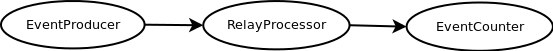
\includegraphics[width=3.0in]{processgraph.png}
	\caption{Process Graph}
	\label{processgraph}
\end{figure}

\subsection{Runtime Graph}
When the system is deployed, there can be multiple instances of a particular stage to handle higher loads making the system scalable. Figure \ref{runtimegraph} shows possible runtime graph for above process graph. Here each parent process instance sends events to two child process instances. However in this case parent process instance has to pick a child process instance to send the message as well. One way of handling this problem is to pick a random node. Another approach is to send messages with same key to same child process instance. 

\begin{figure}[!t]
        \centering
        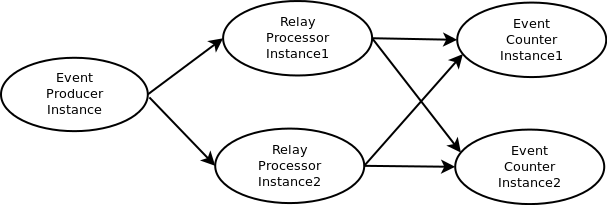
\includegraphics[width=3.0in]{runtimegraph.png}
        \caption{Runtime Graph}
        \label{runtimegraph}
\end{figure}

\subsection{API}
In this section, we explain our API that can be used to define custom events, processes and adapters. We provide clear interfaces to abstract out all the communication complexities from application developers. Table \ref{api} shows details of client interfaces.

\definecolor{dkgreen}{rgb}{0,0.6,0}
\definecolor{gray}{rgb}{0.5,0.5,0.5}
\definecolor{mauve}{rgb}{0.58,0,0.82}

\lstset{frame=tb,
  language=Java,
  aboveskip=3mm,
  belowskip=3mm,
  showstringspaces=false,
  columns=flexible,
  basicstyle={\small\ttfamily},
  numbers=none,
  numberstyle=\tiny\color{gray},
  keywordstyle=\color{blue},
  frame=single,
  breaklines=true,
  breakatwhitespace=true,    
  tabsize=2
}

\begin{table}[ht]
	\centering
	\begin{tabular}{| l | l | l |}
        \hline
        Interface Name &  Method & Parameters \\
        \hline
        Event   & getKey &  \\
        \cline{2-3}
        & serialize &  DataOutput \\
	\cline{2-3}        
        & parse &  DataInput \\
        \hline
        Adapter   & start &  \\
        \cline{2-3}
        & initialize &  Container \\
        \hline
        Processor   & onEvent & Event \\
        \cline{2-3}
        & initialize &  Container \\
        \hline
        \end{tabular}
        \caption{Client API}
        \label{api}
\end{table}


 The \texttt{Event} interface has a method to get the key for a given event. This key is used in sending messages to next processes as described earlier. \texttt{Parse} and \texttt{serialize} methods of \texttt{Event} interface are used to directly serialize the event attributes to underlying streams. When implementing these methods developers can define attribute serialization order in their \texttt{serialize} method and use the same order during \texttt{parse} method to avoid metadata passing with the binary format. \texttt{Processor} interface contains a method called \texttt{onEvent} which is invoked by the underlying framework when it receives an event to that process. The \texttt{start} method of the \texttt{Adapter} interface is invoked by the framework and that can be used to pull events from external systems once the system starts. During initialization both processes and adapters receive the container that can be used to send events to other processes.
 
 \subsection{Deployment}

As shown in Figure \ref{deployment}, a deployment of the system consists of a manager node and a set of worker nodes. Worker nodes are grouped into clusters so that the application users can specify to which clusters each processes needs to get deployed. The Manager node processes applications, deploys them to worker nodes, and initiates the processing by starting the adapters.

\begin{figure}[!t]
        \centering
        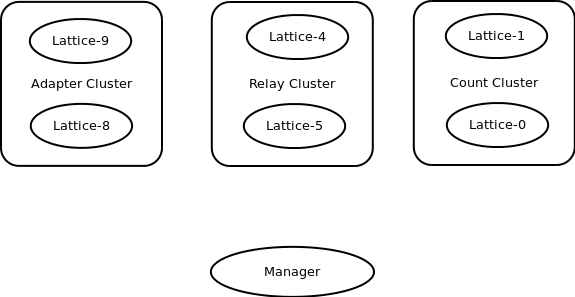
\includegraphics[width=3.0in]{deployment.png}
        \caption{Deployment}
        \label{deployment}
\end{figure}

\subsection{Application Development}

An application specifies the runtime graph to process a particular event stream. Therefore an application mainly consists of a set of processes, adapters and events and their interactions. Processes, adapters and events can be developed by implementing the respective interfaces as shown above. Then the interactions can be specified using a JSON file. 

\lstinputlisting[label=sampleruntime,caption=Runtime Graph,language=java]{runtimegraph.json}

As shown in Listing \ref{sampleruntime}, the \textit{instances} parameter can be used to specify the required number of instances to be deployed. The \textit{receivers} parameter is used to specify from which process it expects to receive messages and how the sending process should distribute the events among instances. The \textit{key} type indicates that the events with the same key must be received by the same instance. Finally users can deploy the application to manager which processes them and deploys to workers.






 

\section{System Design}
In this section we elaborate the underlying system design which is capable of processing 2.4 million messages per second. We emphasize three features of this design. Firstly between any two nodes there is a set of TCP connections (typically 20 connections)  to send messages. All processes share the same set of connections which we called the bridge. The advantage of this approach compared to having TCP connections per process is that it utilizes all available bandwidth even there is only one process per node. However since this is a common bridge now we have to send the receiving process id to dispatch the message, sending  process id to parse the message and sequence number to order messages. As we discuss later our experiments show that this approach perform several times better than the other systems despite the above overhead. Secondly we have implemented \textit{OutputStream} and \textit{InputStream} interfaces on top of java non blocking I/O API. Using these input and output streams we provide \textit{DataOutput} and \textit{DataInput} APIs to directly 
serialize message data to binary format without sending any metadata along the message. Finally except messages themselves, all the other objects used to serialize and parse the messages and parse the messages are not created at message processing time. All these objects are created when a process sends the first message and it is a one-time cost. Rest of this section further explains the design techniques we used to realize these concepts.
\subsection{Inter Process Communication}
Figure \ref{interprocess} shows the design involved in sending a message from one process to another. Lets assume there is a message at a client side process and that process wants to send this message to another process. First the client process sends this message to its \textit{ElementContainer}. \textit{ElementContainer} holds all the streams (this is an abstraction of a link in the process graph) to which this message needs to send and it push the message to all streams. Stream decides which node to send this message and passes the message along the target node details to \textit{ConnectionManager} which holds \textit{ClientConnection}s for each node. \textit{ConnectionManager} sends message to correct \textit{ClientConnection} using target node. \textit{ClientConnection} picks an available \textit{DataOutput} from its pool of \textit{DataOutputs} and invokes the serialize method of the message to send that to server side.

At the server side there is a set of \textit{ServerTask}s which reads receiving messages from a pool of \textit{DataInput} streams available in the \textit{ServerConnection} (we register these connections at the connections creating time). Once a \textit{ServerTask} receives a binary message, it creates the event using the sending process id to identify the event type. Then it passes this message to the \textit{WorkerContainer} which holds all processes. Finally \textit{WorkerContainer} dispatches this message to correct process using receiving process id. Message ordering happens at the process level if required. This illustrates how we have shared a pool of TCP connections among processes and next we show how we have implemented \textit{OutputStream} and \textit{InputStream} with non blocking I/O API without  creating objects dynamically.
\begin{figure}[!tii]
        \centering
        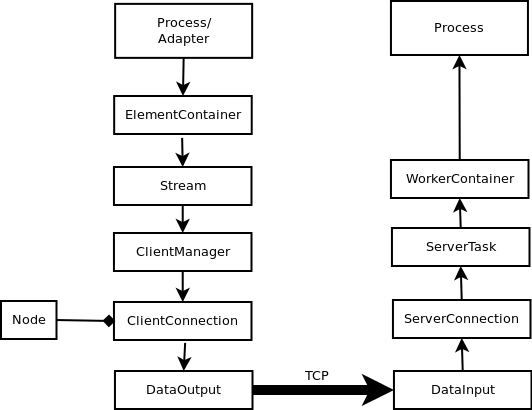
\includegraphics[width=3.0in]{interprocess.png}
        \caption{Communication between two Process}
        \label{interprocess}
\end{figure}
\subsection{Client Side}
Figure \ref{client} shows how we have implemented \textit{OutputStream} interface using our \textit{DataWriter}. \textit{DataWriter} contains a \textit{ByteBuffer}. When a higher layer method writes data to \textit{DataOuput}, \textit{DataWriter} puts those bytes to its byte buffer. When a selection event occurs, \textit{Datawriter} writes its byte buffer to underline \textit{SocketChannel}. This way only one byte buffer is used as an intermediary to create an output stream with non blocking I/O API.
\begin{figure}[!t]
        \centering
        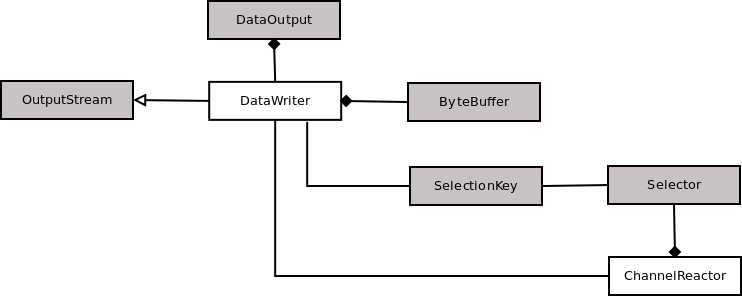
\includegraphics[width=3.0in]{client.png}
        \caption{OutputStream Implementation}
        \label{client}
\end{figure}
\subsection{Server Side}
Figure \ref{server} shows how we have implemented \textit{InputStream} interface using our \textit{DataReader}. Similar to client side, \textit{DataReader} has a \textit{ByteBuffer}. When a selection event occurs \textit{DataReader} inputs bytes from the \textit{SocketChannel} to its byte buffer. When a \textit{ServerTask} reads data through \textit{DataInput}, it reads data from the byte buffer and passes to higher layer. In this way we have implemented an input stream with non blocking I/O API.
\begin{figure}[!t]
        \centering
        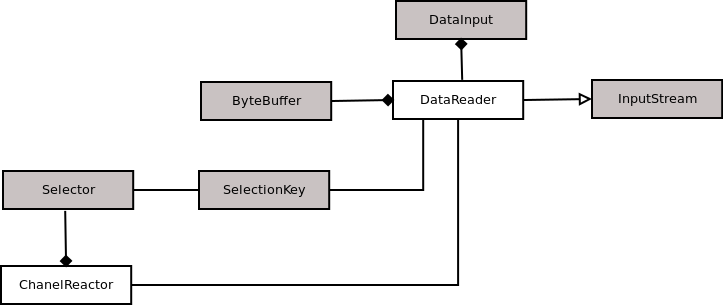
\includegraphics[width=3.0in]{server.png}
        \caption{InputStream Implementation}
        \label{server}
\end{figure}

\section{Experiments}

We conducted several performance tests to measure the throughput and scalability of our system. All these tests were performed in an LAN system called Lattice which has a network bandwidth of 1Gbps. All nodes are Intel(R) Xeon(R) 2.4GHz 4 core duo machines with 1 Gbp of memory. Sample code used for all tests can be found here.

\subsection{Inter node communication}
We used a graph as shown in Figure \ref{ecgGraph} to process ECG signal data. For our solution and Yahoo S4! EventProducer reads a file contains over 7500000 ecg records and push events with multiple threads. Twitter Storm does not allow user threads to push data. So we use the Spout thread to send messages into the system. EventReceiver  receives the ECG events, process them and calculate heart rate interval periodically.  
We execute our system with 1, 2 and 4  EventReceivers for each system and measured the throughput, load average and network bandwidth  for each case. Throughput was measured at the EventProducer calculating total time required to send messages and the total number of messages send. Load average and network bandwidth were measured using top and atop linux commands respectively. Figure \ref{throuput} shows the throughput variation with the number of nodes for all systems. 

\begin{figure}[!t]
        \centering
        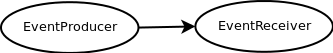
\includegraphics[width=3.0in]{ecgGraph.png}
        \caption{ECG Process Graph}
        \label{ecgGraph}
\end{figure}
\begin{figure}[!t]
        \centering
        \includegraphics[width=3.0in]{throughput.png}
        \caption{Throughput of the systems}
        \label{throuput}
\end{figure}

As shown in the Figure \ref{throuput} our solution out performs Twitter storm and Yahoo S4!. However by looking the Figure \ref{throuput} one might think even our system does not scalable although it perform high. In order to examine the reason behind this we need to look into the network bandwidth and CPU load average values. 
 
Figure \ref{networkandload} shows the network bandwidth usage and the CPU load average at each node. For multiple node scenarios we observed the same values for bandwidth usage and CPU load average at each receiver. Therefore we have taken the average values of them. 

\begin{figure*}[!t]
	\centering
	\subfloat[Network Usage]{\includegraphics[width=3.0in]{network.png}}
	\hfil
	\subfloat[CPU Load Average]{\includegraphics[width=3.0in]{loadaverage.png}}
	\caption{Network usage and CPU Load Average of the System}
	\label{networkandload}
\end{figure*}
 

By looking at the graphs, first it can be observed that our solution utilities all available network bandwidth (98\%) even with two receivers. In only one receiver case, high CPU load average at receiver indicates it has utilized available CPU power. Adding two receivers has increased the CPU power at receiving side utilizing all available network bandwidth. Therefore it can not increase the throughput without increasing network bandwidth although more CPU power available at receiver nodes. Having receiver nodes, we can observe that network bandwidth and CPU load average is reduced at each receiver since load is shared among the receivers. However for other two systems, it neither hits the maximum network bandwidth available nor the full CPU power available at any stage. If a system does not make use of the available resources then adding more resources won't scale up the system. As explained in earlier, our solution utilities all available resources by using parallel tcp connections and having an efficient message parsing technique.

After measuring the throughput we examined the  total amount of extra bytes each system sends to transfer the information from EventProducer to EventReceiver. Our ECGEvent has two double fields called time and value (ecg signal value) and a streamID which is a 4 byte string. So we calculated total bytes to send this information as 20 bytes (16 for two double and 4 for streamID). Then by using the throughput and the bandwidth usage of the system we calculate the total number of bytes each system uses at network layer to send this message. By reducing 20 information bytes we can calculate the over head bytes for each system. Figure \ref{efficiency} compares these numbers.

\begin{figure}[!t]
        \centering
        \includegraphics[width=3.0in]{efficiency.png}

        \caption{Efficiency of Message serialization}
        \label{efficiency}
\end{figure}

As shown in the figure \ref{efficiency} Twitter storm uses a minimum over head while Yahoo S4! performs badly compared to other two. This overhead is due to its usage of  java serializations to serialize data. Then we analyzed to which our solution spends extra 32 bytes. Our solution adds a sequence number (an integer), receiving process id (a 8 byte string for this scenario), sending process id (a 8 byte string for this scenario) to order messages, dispatch the message to correct process and to parse the message at the server. Altogether it adds 26 (serialization format of a string uses two more bytes to keep the string length) extra bytes to each message at application level and other 4 bytes due to tcp over head. This is the trade off we had to pay for improve the parallelism compared to direct one tcp communication per process. 

\subsection{Scalability}
We performed a scalability test for our system using the 3 level graph shown in Figure \ref{multigraph}. The processing data as well as the processing logic were obtained from the Grand Challenge problem of 8th ACM International conference on Distributed Event Based systems. We used the publicly available 500MB of data to generate the events. 

\begin{figure}[!t]
        \centering
        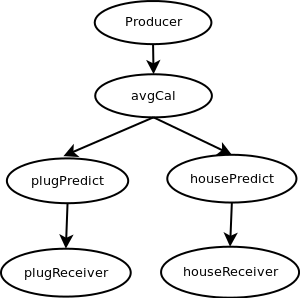
\includegraphics[width=3.0in]{multigraph.png}
        \caption{Multilevel Node Graph}
        \label{multigraph}
\end{figure}

This application predicts load averages using the previous values and a given machine learning algorithm. We implement this logic using nodes as shown in the Figure \ref{multigraph}. First producer reads the data file and send events to the avgCal node which calculate the last minite average and send the same event to both plugPredict and housePredict processors. Both plugPredict and housePredict processors predict the next values and send events to receivers. The original problem only requires to send those prediction events in 30s intervals. But we send a prediction event fore each messages to observe how the system works with high load.
 
As in the earlier case we conduct our experiments using one producer and multiplying the other processing nodes by 1, 2 and 4 times to measure the throughput increase at the producer. We ran each node in a separate machine so that our receiver configurations used 5, 10, 15 machines respectively. We measured the throughput,  network bandwidth and the CPU load average at the producer to examine the scalability of the system. Since the one receiver unit throughput greater than that of the storm one node scenario we only used our system for this experiment.  Results are shown in the Figure \ref{scalability}.

%\begin{figure}
%        \centering
%        \begin{subfigure}[b]{0.45\textwidth}
%                \includegraphics[width=\textwidth]{throughputs.png}
%        \end{subfigure}
%        \begin{subfigure}[b]{0.45\textwidth}
%                \includegraphics[width=\textwidth]{networkps.png}
%        \end{subfigure}
%        \begin{subfigure}[b]{0.45\textwidth}
%                \includegraphics[width=\textwidth]{networks.png}
%        \end{subfigure}
%        \begin{subfigure}[b]{0.45\textwidth}
%                \includegraphics[width=\textwidth]{loadaverages.png}
%        \end{subfigure}
%        \caption{Scalability of the System}
%        \label{scalability}
%\end{figure} 

\begin{figure*}[!t]
        \centering
        \subfloat[Throughput]{\includegraphics[width=3.0in]{throughputs.png}}
        \hfil
        \subfloat[Network Usage]{\includegraphics[width=3.0in]{networkps.png}}
        \hfil
        \subfloat[Network Usage Bandwidth]{\includegraphics[width=3.0in]{networks.png}}
        \hfil
        \subfloat[CPU Load Average]{\includegraphics[width=3.0in]{loadaverages.png}}
        \caption{Scalability of the System}
        \label{scalability}
\end{figure*}


For one receiver unit case, we observed very high load average and network bandwidth usage at avgCal node since it send messages to two nodes. Then as shown in the figure \ref{scalability} we could linerly scale up the system by adding more receiver units to add more cpu power to system. When increasing the receiver units, we can observe throughput of the system increases proportional to number of receiving units. CPU load average of 13 at the producer indicates it has utilized all available CPU power and we need to add more producers to scale this system further up. 



\section{Related Work}
Much of the inspiration for stream processing systems can be trace back to data stream management systems. These systems support a window based query language. Most of these languages are derived from SQL, for instance STREAM\cite{arasu2004stream} defines a language called \textit{Continuous Query Language(CQL)} which has similar syntactic characteristics as SQL. Aurora\cite{abadi2003aurora}, STREAM\cite{arasu2004stream} and Nile\cite{hammad2004nile} are some of the prominent implementations of DSMSs. Complex event processing(CEP) systems such as Esper\cite{esper}, Siddhi\cite{suhothayan2011siddhi}, Cayuga\cite{brenna2007cayuga} also share many characteristics with DSMSs except for their use cases. CEP systems are capable of handling multiple incoming event streams(which are similar to the input streams) and identifying patterns across streams which are of interest to the end users. However these systems does not support user defined logic and hence not suitable for implement complex logic based on machine 
learning techniques. 

Map reduce\cite{dean2008mapreduce} is a widely adapted technology to process batch data with the popularity of Apache Hadoop\cite{hadoop}. In a map reduce environment a problem is partition into smaller parts identified by a key and process parallely. Although these systems support user defined functions, data processing flow of these systems are fixed. Ciel\cite{murray2011ciel} address this problem by dynamically generating data flow graph. Since all these systems communicate through file system they inherently not suitable for real time processing\cite{lam2012muppet}. 

Stream Processing Core (SPC)\cite{Amini2006}, Yahoo S4\cite{neumeyer2010s4} and Twitter Storm\cite{twitterStorm} address the above issue by supporting direct communication. These systems are based on the Actor model\cite{agha1985actors} and each system has a notion of processing element or computation. Processing Elements are used to perform user defined logic on the receiving events and emit newly generated events to other processing elements. In addition to basic communication these systems provide fault tolarance features such as reliable message delivery and dynamic membership management. However most of these system does not focus on improving internode communication performance.

Spark\cite{zaharia2010spark} introduces its RRDs\cite{zaharia2012resilient} to achieve better fault tolerance by storing the operations and replaying them instead of replicating data itself or use checkpointing to store data periodically. Spark Streaming\cite{zaharia2013discretized} extends this concept to distributed stream processing with the concept of discretized events. Spark streaming\cite{zaharia2013discretized} processes data as batches while storing them as RDDs \cite{zaharia2012resilient} to achieve higher throughput. This batch processing may introduce latencies which are not acceptable for some applications. Further it is not clear how to implement complex event processing algorithms such as we use our benchmarks with Spark Streaming. MillWheel\cite{akidau2013millwheel} is the stream processing system used at Google to process web queries. MillWheel\cite{akidau2013millwheel} provides reliable message processing as well as state persistance for its graph based computations. Unlike in our system MillWheel treat messages as binary 
messages leaving message parsing and serialization to application layer. 

\section{Conclusions and Future Work}
In this paper we have described our approach to achieving high-throughput multi-stage stream processing.  We have used application message buffering to improve serialization and deserialization process and thread pools to improve parallelism.

We have validated the soundness of our methodology using empirical benchmarks that contrast its performance with well-known systems such as Twitter Storm \cite{toshniwal2014storm} and Yahoo S4\cite{neumeyer2010s4}. Our approach allows cumulative throughputs that significantly outperform these aforementioned systems. In a two stage setting we are able to achieve a processing throughput of 2.3 million messages per-second and a network utilization of 95\% (950Mbps/1Gbps) even with one receiver. In a four-stage setting we are able to achieve a processing throughput of 2.5 million messages per-second and a network utilization of 98\% (982Mbps/1Gbps) with four receiving units.

Our future work will mainly target two areas: reliable message delivery and compression. We will focus on implementing a reliable message delivery protocol to support at least one guarantee on top of our communication framework.  The work on compression will target reducing the overthe-wire footprints of the packets. We will explore the use of compression algorithms while ensuring that the gains in message size reduction do not result in unacceptable latency overheads and also that the throughput improves. 


% An example of a floating figure using the graphicx package.
% Note that \label must occur AFTER (or within) \caption.
% For figures, \caption should occur after the \includegraphics.
% Note that IEEEtran v1.7 and later has special internal code that
% is designed to preserve the operation of \label within \caption
% even when the captionsoff option is in effect. However, because
% of issues like this, it may be the safest practice to put all your
% \label just after \caption rather than within \caption{}.
%
% Reminder: the "draftcls" or "draftclsnofoot", not "draft", class
% option should be used if it is desired that the figures are to be
% displayed while in draft mode.
%
%\begin{figure}[!t]
%\centering
%\includegraphics[width=2.5in]{myfigure}
% where an .eps filename suffix will be assumed under latex, 
% and a .pdf suffix will be assumed for pdflatex; or what has been declared
% via \DeclareGraphicsExtensions.
%\caption{Simulation Results}
%\label{fig_sim}
%\end{figure}

% Note that IEEE typically puts floats only at the top, even when this
% results in a large percentage of a column being occupied by floats.


% An example of a double column floating figure using two subfigures.
% (The subfig.sty package must be loaded for this to work.)
% The subfigure \label commands are set within each subfloat command, the
% \label for the overall figure must come after \caption.
% \hfil must be used as a separator to get equal spacing.
% The subfigure.sty package works much the same way, except \subfigure is
% used instead of \subfloat.
%
%\begin{figure*}[!t]
%\centerline{\subfloat[Case I]\includegraphics[width=2.5in]{subfigcase1}%
%\label{fig_first_case}}
%\hfil
%\subfloat[Case II]{\includegraphics[width=2.5in]{subfigcase2}%
%\label{fig_second_case}}}
%\caption{Simulation results}
%\label{fig_sim}
%\end{figure*}
%
% Note that often IEEE papers with subfigures do not employ subfigure
% captions (using the optional argument to \subfloat), but instead will
% reference/describe all of them (a), (b), etc., within the main caption.


% An example of a floating table. Note that, for IEEE style tables, the 
% \caption command should come BEFORE the table. Table text will default to
% \footnotesize as IEEE normally uses this smaller font for tables.
% The \label must come after \caption as always.
%
%\begin{table}[!t]
%% increase table row spacing, adjust to taste
%\renewcommand{\arraystretch}{1.3}
% if using array.sty, it might be a good idea to tweak the value of
% \extrarowheight as needed to properly center the text within the cells
%\caption{An Example of a Table}
%\label{table_example}
%\centering
%% Some packages, such as MDW tools, offer better commands for making tables
%% than the plain LaTeX2e tabular which is used here.
%\begin{tabular}{|c||c|}
%\hline
%One & Two\\
%\hline
%Three & Four\\
%\hline
%\end{tabular}
%\end{table}


% Note that IEEE does not put floats in the very first column - or typically
% anywhere on the first page for that matter. Also, in-text middle ("here")
% positioning is not used. Most IEEE journals/conferences use top floats
% exclusively. Note that, LaTeX2e, unlike IEEE journals/conferences, places
% footnotes above bottom floats. This can be corrected via the \fnbelowfloat
% command of the stfloats package.

\section{Acknowledgement}
This research is supported by a grant from the US National Science Foundation's Computer
Systems Research Program (CNS-1253908).

% conference papers do not normally have an appendix


% trigger a \newpage just before the given reference
% number - used to balance the columns on the last page
% adjust value as needed - may need to be readjusted if
% the document is modified later
%\IEEEtriggeratref{8}
% The "triggered" command can be changed if desired:
%\IEEEtriggercmd{\enlargethispage{-5in}}

% references section

% can use a bibliography generated by BibTeX as a .bbl file
% BibTeX documentation can be easily obtained at:
% http://www.ctan.org/tex-archive/biblio/bibtex/contrib/doc/
% The IEEEtran BibTeX style support page is at:
% http://www.michaelshell.org/tex/ieeetran/bibtex/
%\bibliographystyle{IEEEtran}
% argument is your BibTeX string definitions and bibliography database(s)
%\bibliography{IEEEabrv,../bib/paper}
%
% <OR> manually copy in the resultant .bbl file
% set second argument of \begin to the number of references
% (used to reserve space for the reference number labels box)
%\begin{thebibliography}{1}

%\bibitem{IEEEhowto:kopka}
%H.~Kopka and P.~W. Daly, \emph{A Guide to \LaTeX}, 3rd~ed.\hskip 1em plus
%  0.5em minus 0.4em\relax Harlow, England: Addison-Wesley, 1999.

%\end{thebibliography}
\bibliography{paper}
\bibliographystyle{ieeetr}



% that's all folks
\end{document}


